% Data split and model-validation protocol (Section 3.3).
\documentclass[tikz,border=1pt]{standalone}
% =====================================================================
%  Shared style for every diagram in the proposal.
%  Each figure is a standalone TikZ file that \input's this preamble, so
%  all diagrams use the same font family (Computer Modern, T1 -- identical
%  to the LLNCS body text), the same sizes and the same palette.
%
%  Font rule (do not change per figure):
%    node text   \footnotesize  (8 pt)
%    edge labels \scriptsize    (7 pt)
%    titles      \footnotesize\bfseries
%  Figures are drawn at their final width (<= 12.2 cm, the LLNCS text
%  width) and included WITHOUT scaling, so the printed size is the same
%  in every figure.
% =====================================================================
\usepackage[T1]{fontenc}
\usepackage{amsmath,amssymb}
\usepackage{xcolor}
\usepackage{tikz}
\usetikzlibrary{positioning,arrows.meta,shapes.geometric,shapes.multipart,
  fit,backgrounds,calc,shadows,patterns}

% ---- palette ---------------------------------------------------------
\definecolor{cBlue}{HTML}{0B4F8A}    % application / API
\definecolor{cOrange}{HTML}{B4540A}  % processing / services
\definecolor{cPurple}{HTML}{5B3CC4}  % data stores
\definecolor{cGreen}{HTML}{1B7A3A}   % success / output
\definecolor{cRed}{HTML}{B42318}     % error / risk
\definecolor{cGray}{HTML}{5F6672}    % external / neutral
\definecolor{cInk}{HTML}{1F2933}     % text and arrows

\colorlet{fBlue}{cBlue!9}
\colorlet{fOrange}{cOrange!10}
\colorlet{fPurple}{cPurple!9}
\colorlet{fGreen}{cGreen!10}
\colorlet{fRed}{cRed!9}
\colorlet{fGray}{cGray!8}

% ---- fonts -----------------------------------------------------------
\newcommand{\figfont}{\footnotesize}
\newcommand{\lblfont}{\scriptsize}
\newcommand{\code}[1]{\texttt{#1}}

\tikzset{
  every picture/.style={font=\figfont, line join=round, >={Stealth[length=4pt,width=3.4pt]}},
  every node/.append style={execute at begin node={\hyphenpenalty=10000\exhyphenpenalty=10000}},
  base/.style={draw, rounded corners=2pt, line width=0.6pt, align=center,
               inner xsep=3pt, inner ysep=2.5pt, text=cInk, font=\figfont},
  app/.style={base, draw=cBlue, fill=fBlue},
  svc/.style={base, draw=cOrange, fill=fOrange},
  data/.style={base, draw=cPurple, fill=fPurple},
  ok/.style={base, draw=cGreen, fill=fGreen},
  bad/.style={base, draw=cRed, fill=fRed},
  ext/.style={base, draw=cGray, fill=fGray},
  plain/.style={base, draw=none, fill=none},
  db/.style={cylinder, shape border rotate=90, aspect=0.22, draw=cPurple,
             fill=fPurple, line width=0.6pt, align=center, text=cInk,
             minimum height=9mm, font=\figfont},
  decision/.style={diamond, aspect=2.2, draw=cOrange, fill=fOrange,
                   line width=0.6pt, align=center, inner sep=1pt, text=cInk, font=\figfont},
  actor/.style={draw=cInk, fill=fGray, line width=0.8pt, rounded corners=0pt,
                align=center, inner sep=3pt, font=\figfont\bfseries},
  layer/.style={draw=cGray!60, fill=cGray!4, rounded corners=3pt, line width=0.5pt},
  layertitle/.style={font=\lblfont\bfseries, text=cGray, anchor=north west, inner sep=2pt},
  arr/.style={->, draw=cInk, line width=0.6pt},
  darr/.style={->, draw=cGray, line width=0.6pt, dashed},
  biarr/.style={<->, draw=cInk, line width=0.6pt},
  lbl/.style={font=\lblfont, text=cInk, inner sep=1.5pt},
  lblbg/.style={font=\lblfont, text=cInk, inner sep=1.5pt, fill=white},
}

% ---- UML sequence-diagram helpers -----------------------------------
%  \lifeline{id}{x}{label}{bottom y}   head box + dashed life line
%  \msg{x1}{x2}{y}{label}              synchronous call (solid)
%  \ret{x1}{x2}{y}{label}              reply (dashed)
%  \selfmsg{x}{y}{label}               call to self, label on the right
%  \fragment{kind}{guard}{x1}{y1}{x2}{y2}  combined fragment (alt/loop/par)
\newcommand{\lifeline}[4]{%
  \node[app, text width=19mm, minimum height=8.5mm, font=\figfont\bfseries] (#1) at (#2,0) {#3};
  \draw[cGray, dashed, line width=0.5pt] (#1.south) -- (#2,#4);}
\newcommand{\msg}[4]{%
  \draw[arr] (#1,#3) -- node[lbl, above] {#4} (#2,#3);}
\newcommand{\ret}[4]{%
  \draw[darr] (#1,#3) -- node[lbl, above] {#4} (#2,#3);}
\newcommand{\selfmsg}[3]{%
  \draw[arr] (#1,#2+0.12) -- ++(0.3,0) -- ++(0,-0.24) -- ++(-0.3,0);
  \node[lbl, anchor=west, align=left] at (#1+0.35,#2) {#3};}
\newcommand{\fragment}[6]{%
  \draw[cGray, line width=0.5pt] (#3,#4) rectangle (#5,#6);
  \node[anchor=north west, draw=cGray, fill=white, font=\lblfont\bfseries,
        inner sep=1.5pt, line width=0.5pt] at (#3,#4) {#1};
  \if\relax\detokenize{#2}\relax\else
  \node[anchor=north west, font=\lblfont, text=cGray, inner sep=1.5pt] at (#3+0.75,#4) {[#2]};\fi}
\newcommand{\activation}[3]{% x, y top, y bottom
  \draw[draw=cBlue, fill=fBlue, line width=0.5pt] (#1-0.07,#2) rectangle (#1+0.07,#3);}

\begin{document}
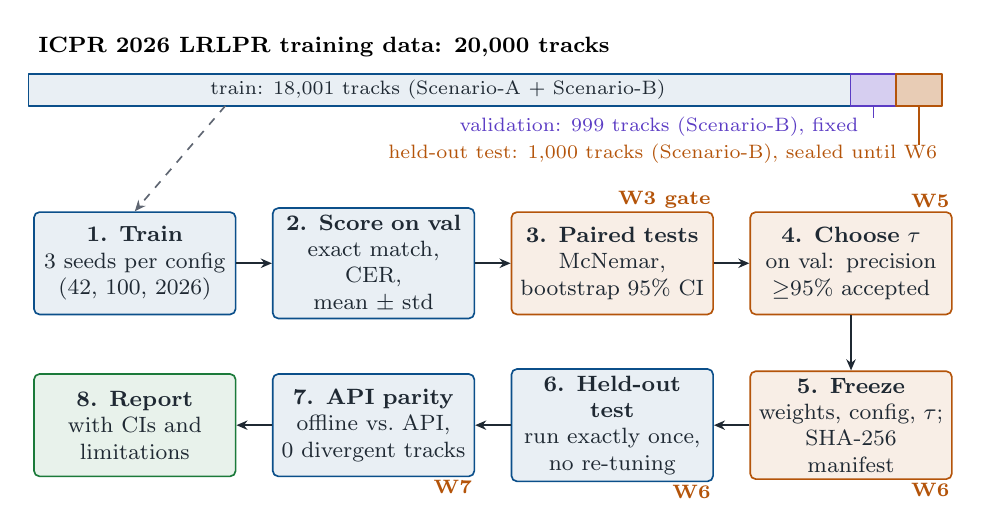
\begin{tikzpicture}
  \tikzset{pstep/.style={app, text width=23.5mm, minimum height=13mm},
           gate/.style={svc, text width=23.5mm, minimum height=13mm},
           wk/.style={font=\lblfont\bfseries, text=cOrange, anchor=south east, inner sep=1pt}}
  % ---------------- data split (to scale) ----------------
  \node[font=\figfont\bfseries, anchor=west] at (0,0.75) {ICPR 2026 LRLPR training data: 20{,}000 tracks};
  \draw[draw=cBlue, fill=fBlue, line width=0.6pt] (0,0) rectangle (10.44,0.4);
  \draw[draw=cPurple, fill=cPurple!25, line width=0.6pt] (10.44,0) rectangle (11.02,0.4);
  \draw[draw=cOrange, fill=cOrange!30, line width=0.6pt] (11.02,0) rectangle (11.6,0.4);
  \node[lbl] at (5.2,0.2) {train: 18{,}001 tracks (Scenario-A + Scenario-B)};
  \node[lbl, anchor=north east, align=right, text=cPurple] (vl) at (10.6,-0.08) {validation: 999 tracks (Scenario-B), fixed};
  \node[lbl, anchor=north east, align=right, text=cOrange] (hl) at (11.6,-0.42) {held-out test: 1{,}000 tracks (Scenario-B), sealed until W6};
  \draw[cPurple, line width=0.5pt] (10.73,0) -- (10.73,-0.15);
  \draw[cOrange, line width=0.5pt] (11.31,0) -- (11.31,-0.5);

  % ---------------- protocol ----------------
  \node[pstep] (s1) at (1.35,-2.0) {\textbf{1. Train}\\3 seeds per config\\(42, 100, 2026)};
  \node[pstep, right=4.5mm of s1] (s2) {\textbf{2. Score on val}\\exact match, CER,\\mean $\pm$ std};
  \node[gate, right=4.5mm of s2] (s3) {\textbf{3. Paired tests}\\McNemar,\\bootstrap 95\% CI};
  \node[gate, right=4.5mm of s3] (s4) {\textbf{4. Choose $\tau$}\\on val: precision\\$\ge$95\% accepted};
  \node[gate, below=7mm of s4] (s5) {\textbf{5. Freeze}\\weights, config, $\tau$;\\SHA-256 manifest};
  \node[pstep, left=4.5mm of s5] (s6) {\textbf{6. Held-out test}\\run exactly once,\\no re-tuning};
  \node[pstep, left=4.5mm of s6] (s7) {\textbf{7. API parity}\\offline vs.\ API,\\0 divergent tracks};
  \node[ok, text width=23.5mm, minimum height=13mm, left=4.5mm of s7] (s8) {\textbf{8. Report}\\with CIs and\\limitations};
  \foreach \a/\b in {s1/s2,s2/s3,s3/s4,s4/s5,s5/s6,s6/s7,s7/s8} \draw[arr] (\a) -- (\b);
  \node[wk] at (s3.north east) {W3 gate};
  \node[wk] at (s4.north east) {W5};
  \node[wk] at (s5.south east) [anchor=north east] {W6};
  \node[wk] at (s6.south east) [anchor=north east] {W6};
  \node[wk] at (s7.south east) [anchor=north east] {W7};
  \draw[darr] (2.5,0) -- (s1.north);
\end{tikzpicture}
\end{document}
